\section{The Method of Green's Functions}
\setcounter{example}{0}
\subsection{Introduction}
    A \df{Green's function} is the solution to a differential equation of the form
    \begin{equation} \label{eq:greensdef}
        \opp{L^*_\xi} G(\xi, x) = \delta(\xi - x)
    \end{equation}
    satisfying boundary conditions related to those applied to the function of interest.
    The subscript \(\xi\) on the differential operator indicates that the derivatives are being taken with respect to the variable \(\xi\). By making use of some of the delta function's unusual properties, Green's functions can be used to solve nonhomogeneous linear differential equations.

    To find the solution to the linear differential equation
    \begin{equation} \label{eq:4.2}
        \opp{L}u=\phi,
    \end{equation}
    we start by finding the formal adjoint as in equation (\ref{eq:adjoint}). If we replace \(v\) with \(G\), and we replace \(x\) with a dummy variable \(\xi\), we are left with an equation of the form
    \begin{equation} \label{eq:greenadjoint}
        \intl G(\xi, x)\opp{L}u(\xi) d\xi = \bterms + \intl u(\xi)\opp{L^*}G(\xi,x) d\xi.
    \end{equation} 
    It follows from equation (\ref{eq:greensdef}) that we can replace \(\opp{L^*}G\) with \(\d\), and from equation (\ref{eq:4.2}) that we can replace \(\opp{L}u\) with \(\phi\), 
    \begin{equation}
        \begin{split}
            \intl G(\xi,x)\phi(\xi) d\xi &= \bterms + \intl u(\xi)\d(\xi-x) d\xi\\
            &=\bterms + u(x).
        \end{split}
    \end{equation}
    Therefore, if we choose boundary conditions for \(G\) such that the boundary terms do not depend on \(u\) and we are able to find \(G\), then finding \(u\) is reduced to a problem of integrating \(G\phi\). 

    To illustrate the key ideas of the method, we will consider several examples which begin simply and become more complex. Each example will be concerned with a key concept in implementing the method of Green's functions.

\subsection{Example 1 \textit{Loaded String}}
    
    Consider the boundary value problem
    \begin{equation} \label{ex1:initialize}
        u''(x) = \phi(x);\quad u(0)=u(1)=0
    \end{equation}
    where \(\phi(x)\) is prescribed. Equation (\ref{ex1:initialize}) can be regarded as describing the static deflection of a string under unit tension between fixed endpoints and subjected to a force distribution \(\phi(x)\).

    To show that this differential equation does describe the loaded string, we first assume \(|u(x)|<<1\). Then, consider a local area of the deflected string which has tension, \(\bf{T_1}\), in one direction and tension, \(T_2\), in the other, and a small amount of mass downward (Figure 4.1). We draw a free-body diagram for this in Figure 4.2. We can see that via Newton's second law of motion,
    \begin{equation*}
        \begin{split}
            \Sigma \mathbf{F} &= m\opp{a}\\
            \opp{T_1} + \opp{T_2} + dm\opp{g} = 0
        \end{split}
    \end{equation*}
    In the \(x\) direction that is,
    \begin{equation}\label{eq:xdir}
        -T_1\cos \theta_1 + T_2 \cos\theta_2 = 0,
    \end{equation}
    and in the \(y\) direction
    \begin{equation}\label{eq:ydir}
        -T_1\sin\theta_1 + T_2\sin\theta_2 = dm\opp{g}.
    \end{equation}
    Because the deflection of the string is small, \(\theta_1\) and \(\theta_2\) must be much less than 1, and so by the small angle approximation,
    \begin{equation*}
        \cos \theta_1 \approx \cos \theta_2 \approx 1,
    \end{equation*}
    and therefore, from equation (\ref{eq:xdir}), \(T_1=T_2=T\). Also, by the small angle approximation \(\tan \theta\approx u'(x)\). Additionally, \(dmg = \rho g ds\) where \(ds\) is a small element of arc length, so 
    \begin{equation*}
        \begin{split}
            ds &= \sqrt{(dx)^2 + (u')^2dx}\\
            &\approx dx.
        \end{split}
    \end{equation*}
    
    Applying this to equation (\ref{eq:ydir}), we see that 
    \begin{equation*}
        \begin{split}
            T(\tan\theta_2-\tan\theta_1) &\approx \phi ds\\
            T(u'(x_2)-u'(x_1)) & \approx \phi dx\\
            \frac{u'(x_2)-u'(x_1)}{dx} &\approx \frac{\phi}{T},\quad \text{Let } T=1\\
            u''(x)&\approx \phi(x).
        \end{split}
    \end{equation*}
    \begin{figure}
        \centering
        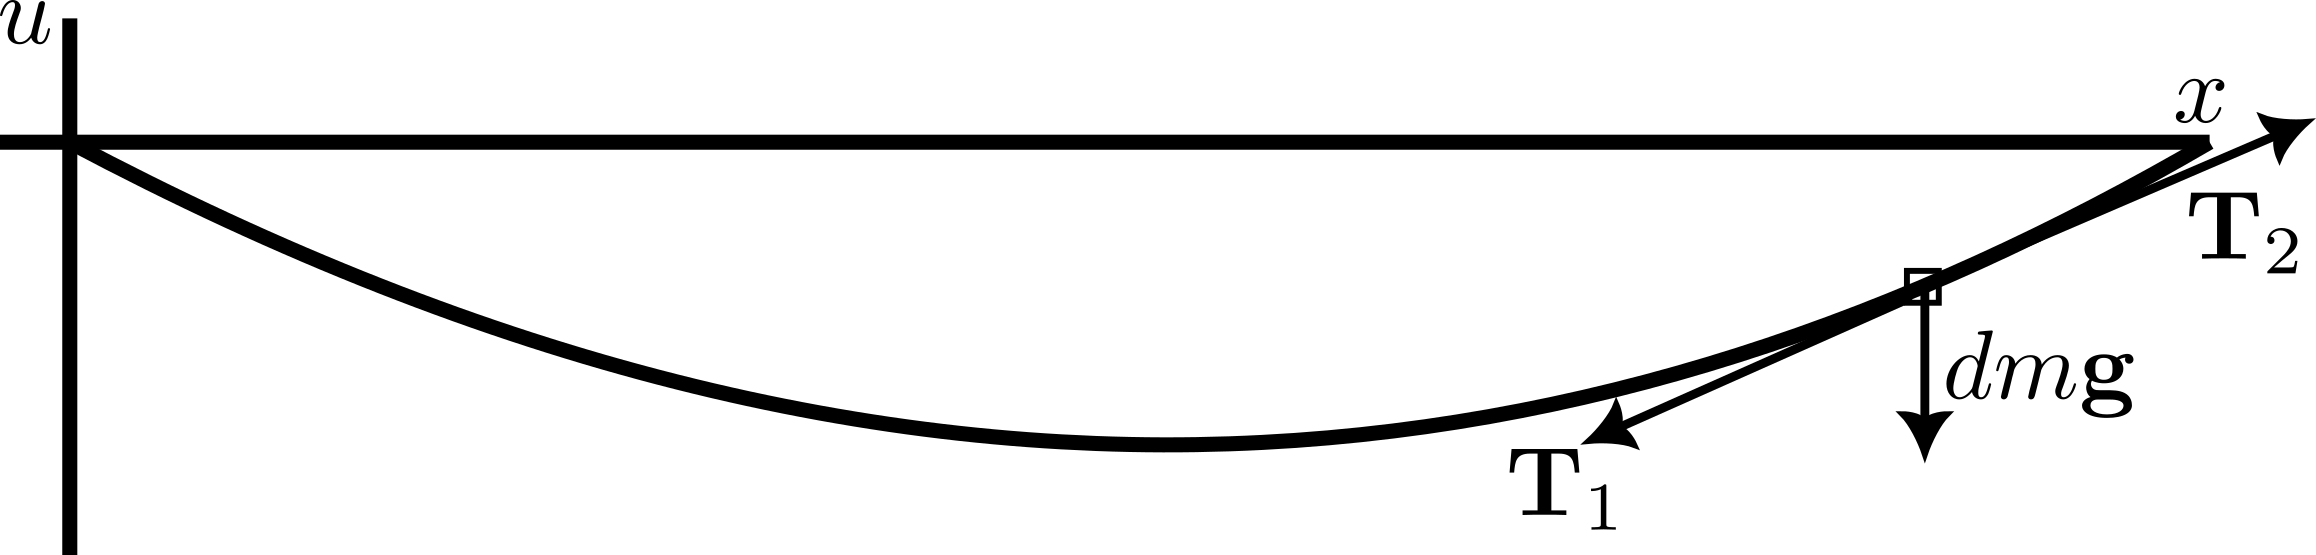
\includegraphics[width=0.6\linewidth]{include/loadtension1.png}
        \caption{Loaded string with tensions.}
    \end{figure}

    \begin{figure}
        \centering
        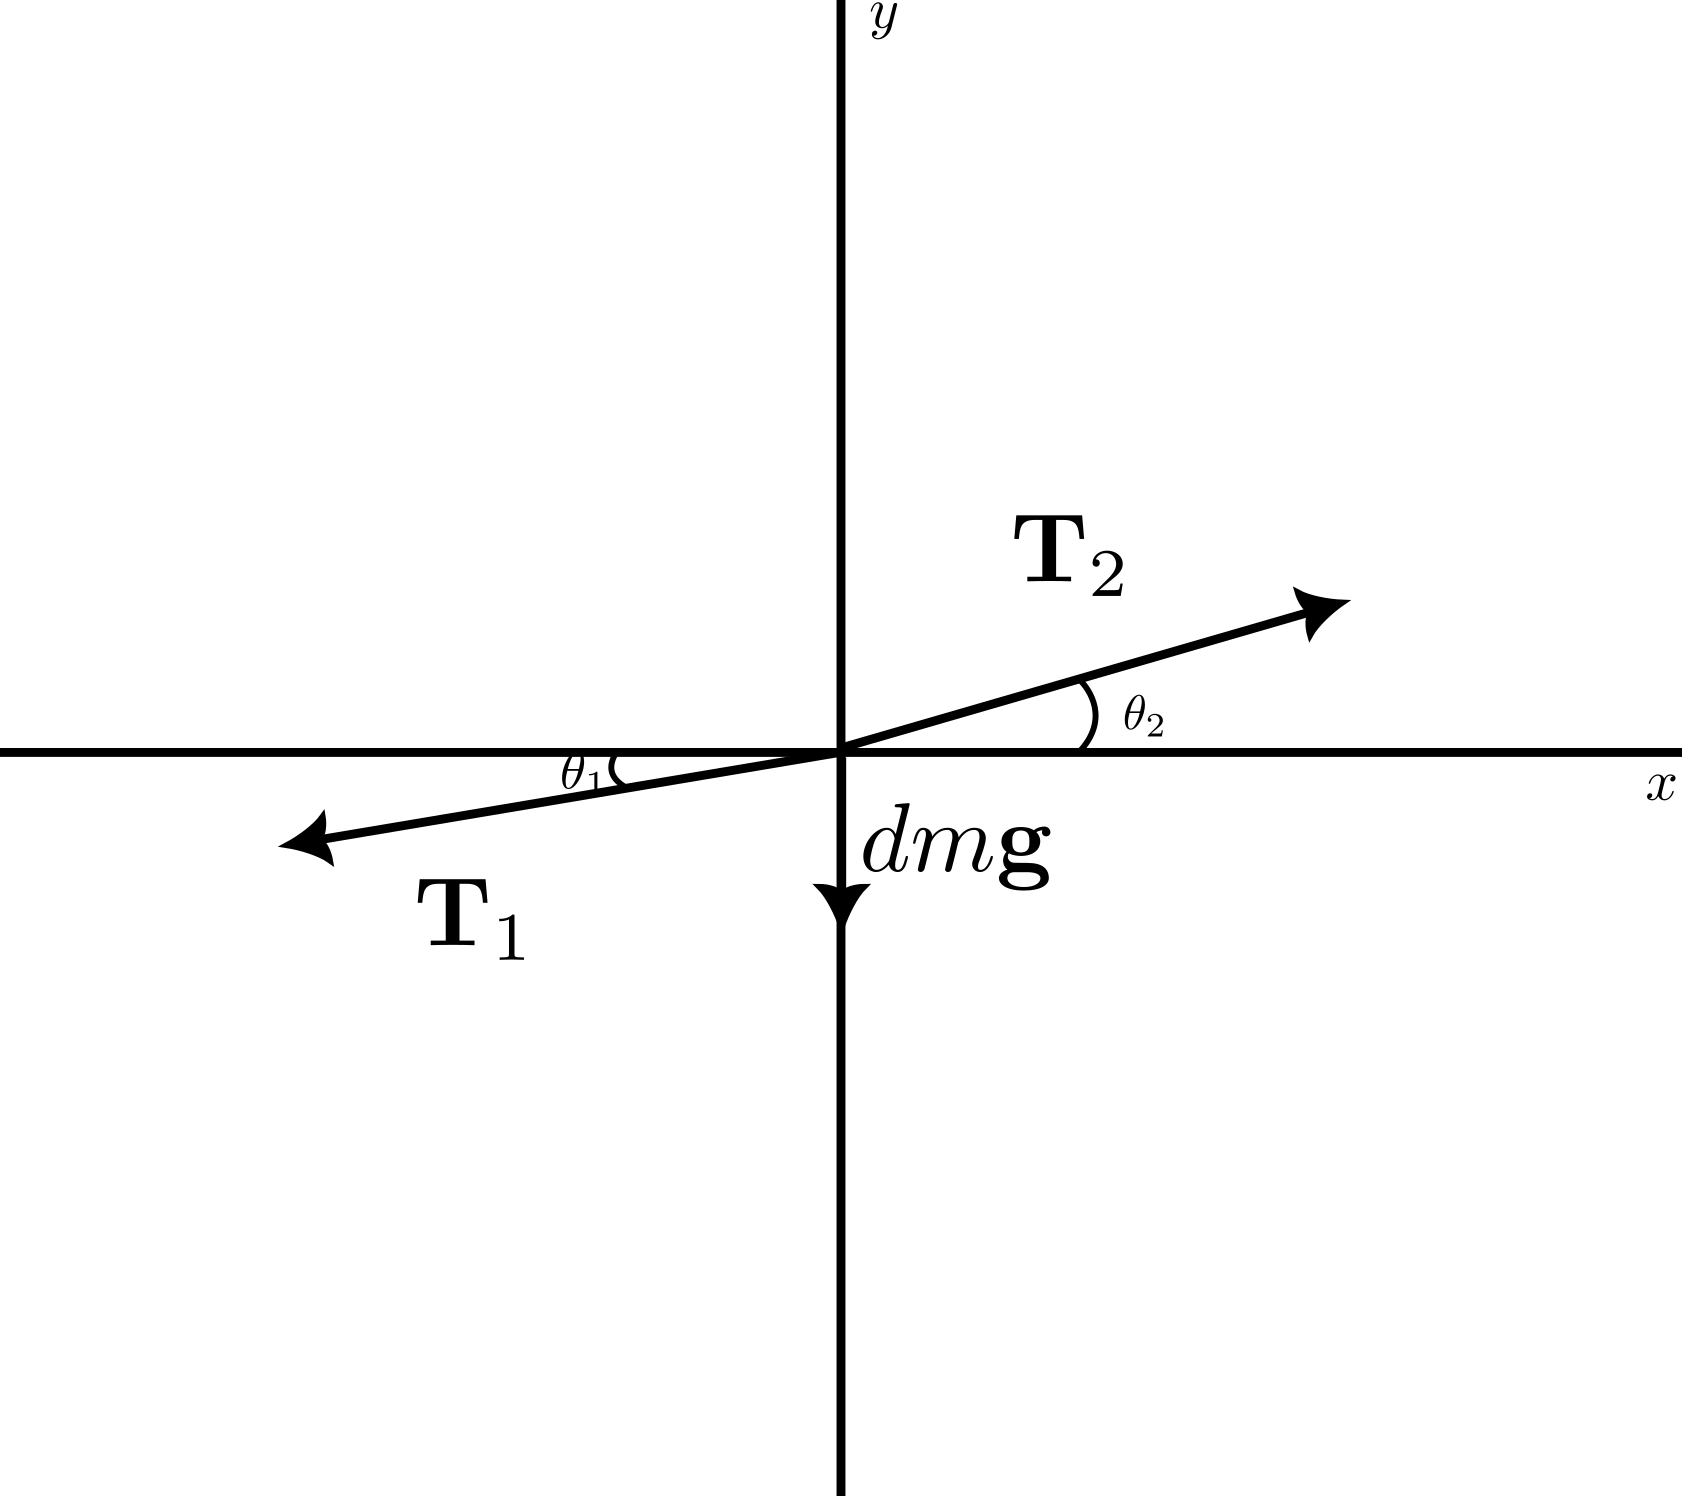
\includegraphics[width=0.6\linewidth]{include/loadtension2.png}
        \caption{Loaded string free-body diagram.}
    \end{figure}

    \begin{figure}\label{fig:LoadedString}
    \centering
    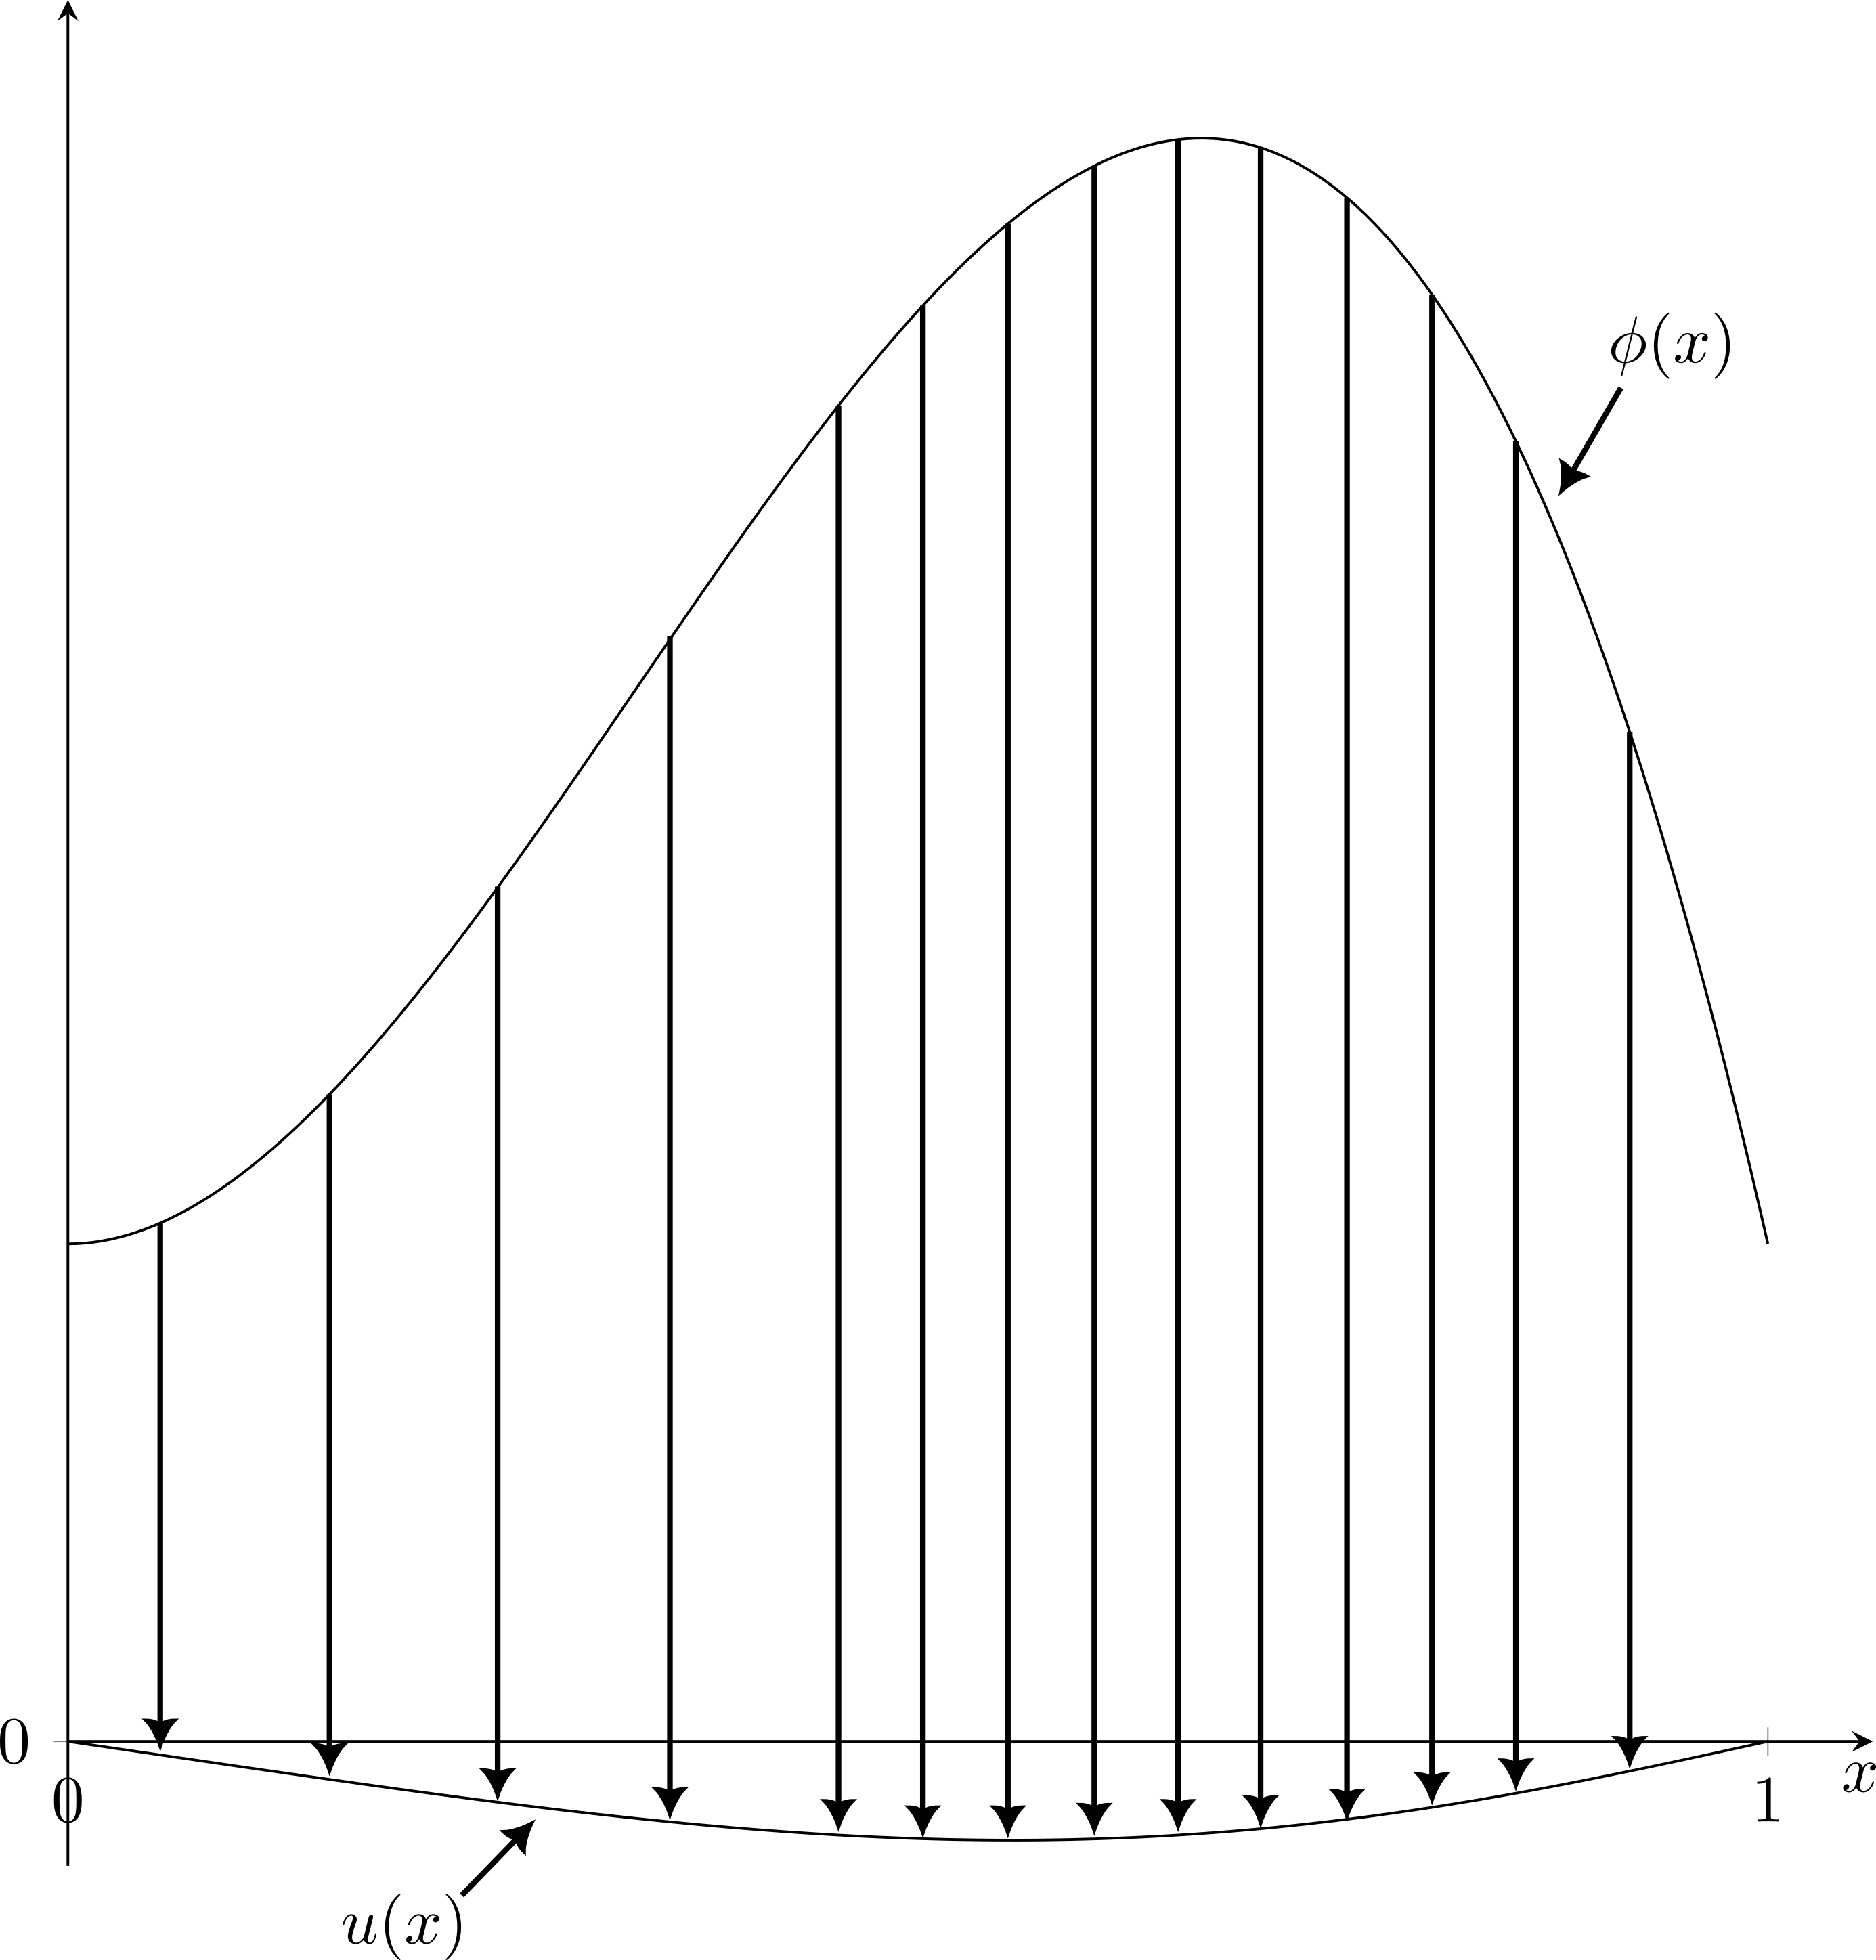
\includegraphics[width=0.5\linewidth]{include/loadedstring.png}
    \caption{Loaded String}
\end{figure}
    
    To find a solution to this differential equation, we first find the formal adjoint \(\Lstar\) as in equation~(\ref{eq:greenadjoint}), 
    \begin{equation}
        \begin{split}
            \int_{0}^{1} G(\xi, x)\L u(\xi) d\xi  &= (G(\xi, x)u'(\xi)-G_\xi (\xi, x)u(\xi))\biggr\rvert_0^1 + \int_{0}^{1} uG_{\xi\xi}d\xi\\
            &= G(1, x)u'(1) - G_\xi(1, x)u(1) \\&- G(0, x)u'(0) + G_\xi(0,x)u(0) + \int_{0}^{1} uG_{\xi\xi}d\xi.
        \end{split}
    \end{equation}
    Therefore, 
    \begin{equation}
        \Lstar = \frac{d^2}{d\xi^2}
    \end{equation}
    and 
    \begin{equation}\label{eq:loadedStringLstarG}
        \Lstar G = G_{\xi\xi} = \delta(\xi-x).
    \end{equation}
    Because of the boundary conditions on \(u\) in equation (\ref{ex1:initialize}), two of our boundary terms are zero. Thus,
    \begin{equation}
        \int_{0}^{1} G(\xi, x)\L u(\xi) d\xi = G(1, x)u'(1) - G(0, x)u'(0) + \int_{0}^{1} uG_{\xi\xi}d\xi.
    \end{equation}
    Now, we want to remove the \(u\) dependency from the boundary terms and, as such, impose the conditions that
    \begin{equation}\label{eq:LoadedstringGBounds}
        G(1,x) = G(0,x) = 0.
    \end{equation}
    Then, provided we can find \(G\) satisfying equations (\ref{eq:loadedStringLstarG}) and (\ref{eq:LoadedstringGBounds}),the solution is given by 
    \begin{equation}\label{eq:loadSln}
        u(x) = \int_0^1 G(\xi,x)\phi(\xi)d\xi.
    \end{equation}
    To find the Green's function, we integrate equation (\ref{eq:loadedStringLstarG}), regarding \(x\) as fixed.
    \begin{equation}
        \begin{split}
            G_\xi &= H(\xi-x) + A(x)\\
            G &= (\xi - x)H(\xi-x)+A(x)\xi +B(x)
        \end{split}
    \end{equation}
    Imposing the boundary conditions, 
    \begin{equation}
        \begin{split}
            &G(0,x) = 0 = B(x)\\
            &G(1,x) = 0 =  1 - x + A(x) + B(x),
        \end{split}
    \end{equation}
    shows us that \(B(x)=0\) and  \(A(x)=x-1\). Therefore
    \begin{equation}\label{eq:LoadGf}
        G(\xi,x) = (\xi-x)H(\xi-x) + (x-1)\xi.
    \end{equation}

    Equation (\ref{eq:loadedStringLstarG}) can, like equation (\ref{ex1:initialize}), be interpreted as the deflection of a loaded string. Specifically, it is the deflection as a function of \(\xi\) due to a point load of unit strength at \(x=\x\), \(\d(\xi-x)\), instead of a load distribution, \(\phi\). Rewriting our Green's function as
    \begin{equation}
        G(\xi,x)= \begin{cases}
            (x-1)\xi, & \xi \leq x\\
            (\xi-1)x, & > \geq x
        \end{cases}
    \end{equation}
    makes it clear that \(G(\xi,x)\) is symetric, to wit: \(G(\xi,x)=G(x,\xi)\). This is often referred to as ``Maxwell Reciprocity.'' Because of this reciprocity, \(G(\xi,x)\) is also the deflection, as a function of \(x\), due to a unit load at \(\xi\). Then, \(G(\xi,x)\phi(\xi)d\xi\) is the deflection due to an incremental load \(\phi(\xi)d\xi\) at \(\xi\). As such, equation (\ref{eq:loadSln}) represents the superposition of these deflections. It is important to recognize that the superposition nature of equation (\ref{eq:loadSln}) is a result of the linearity of \(\mathcal{L}\).

    Additionally, it should be noted that the boundary terms do not always vanish. For example, if we change the boundary condition \(u(1)=0\) to \(u(1)=\a\), then
    \begin{equation*}
        u(x)=\a x + \int_{0}^{1} G(\xi,x)\phi(\xi)d\xi.
    \end{equation*}
    Here, \(G\) is still given by equation (\ref{eq:LoadGf}) because changing the boundary conditions on \(u\) in this way, does not change that the boundary conditions on \(G\) need to be such that 
    \begin{equation*}
        G(0,x)u'(0) = 0 \text{ and } G(1,x)u'(1)=0.
    \end{equation*}

    \subsection{Example 2 \textit{Infinite Beam on an Elastic Foundation}}
    It is prudent to, next, consider a differential operator defined over an infinite interval. We imagine an infinitely long beam on an elastic foundation. According to the classical Euler beam theory, the deflection, \(u(x)\), resulting from a net loading, \(p(x)\) force per unit length, satisfies the differential equation
    \begin{equation*}\label{eq:loadedStringStart}
        (EIu'')'' = p(x).
    \end{equation*}
    \begin{figure}
        \centering
        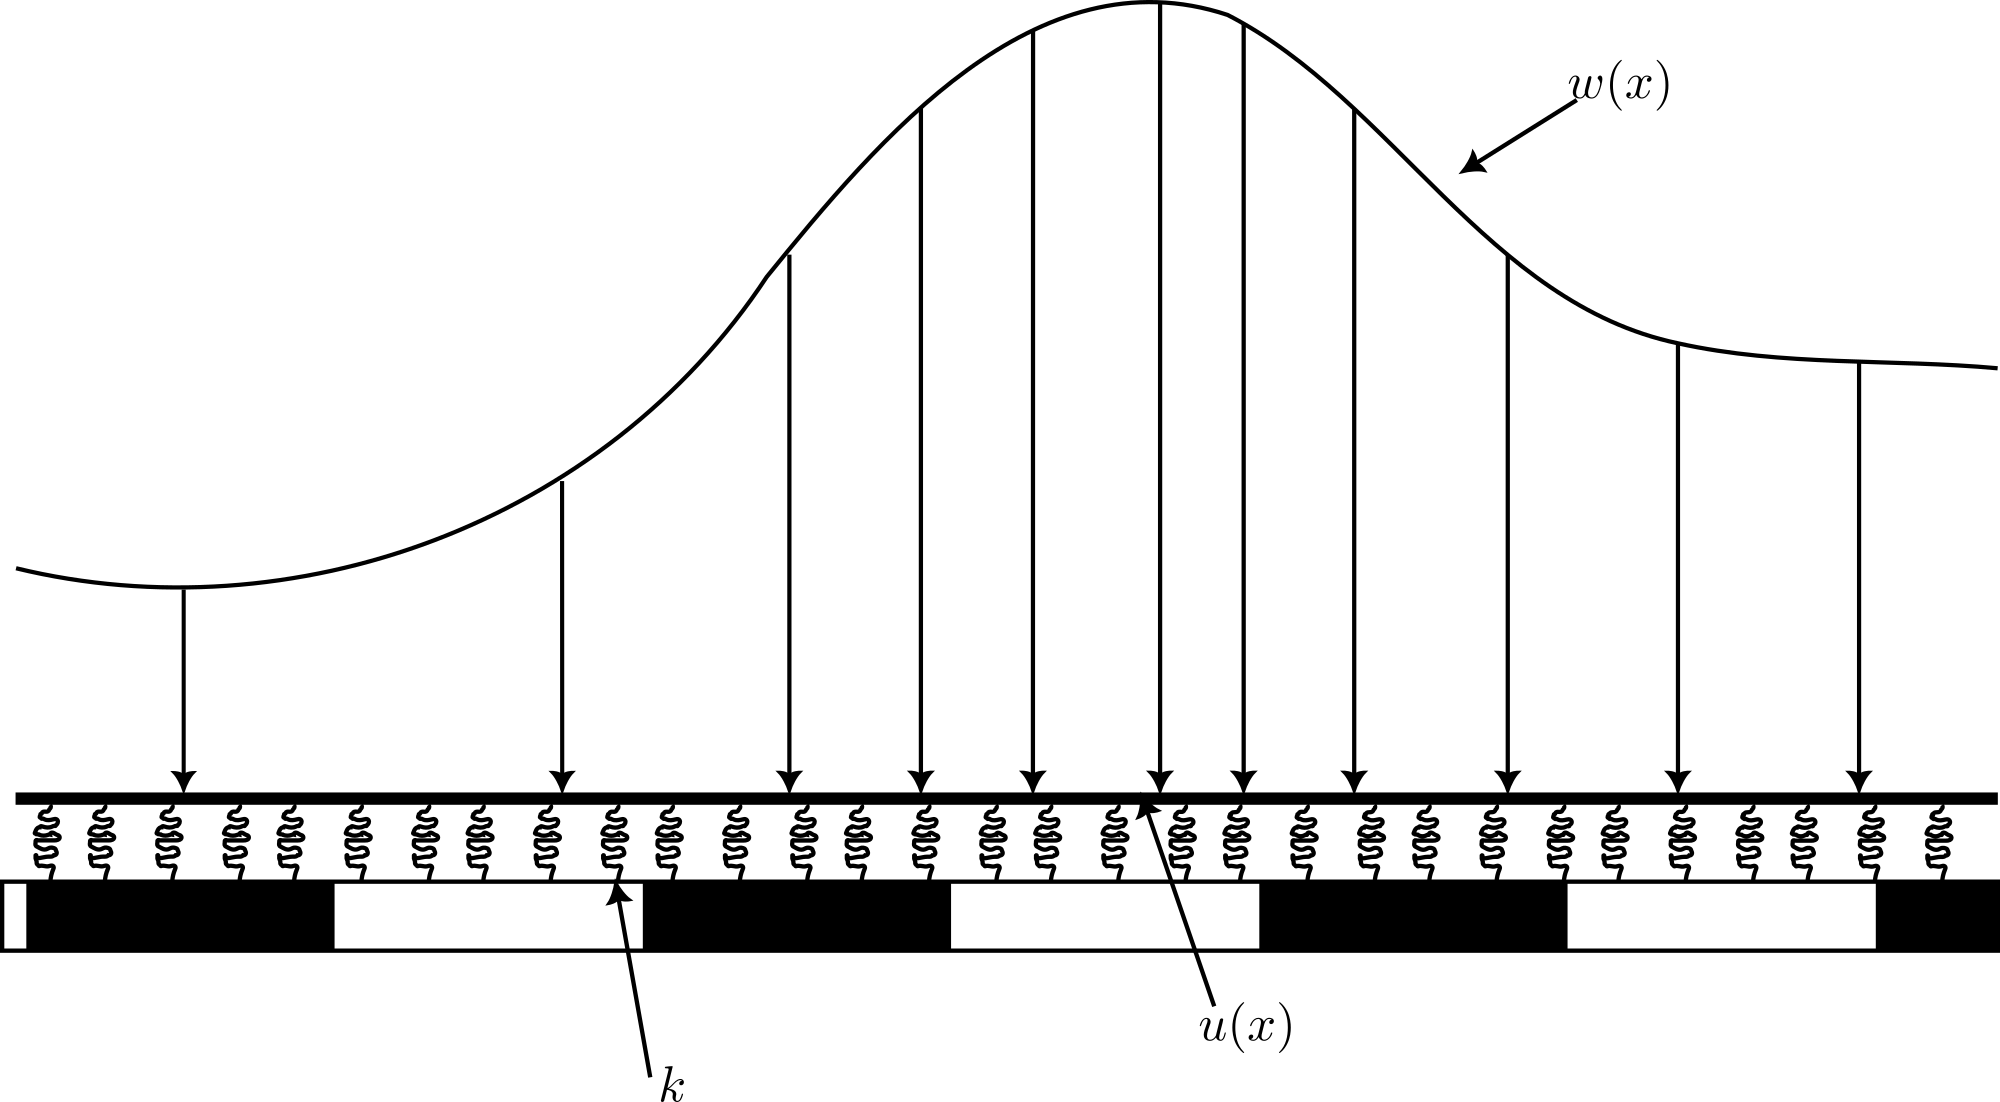
\includegraphics[width=0.75\linewidth]{include/Beam.png}
        \caption{Infinite beam on elastic foundation}
    \end{figure}

    Where the flexural rigidity of the beam, \(EI\), may be a function of \(x\). We also consider the spring constant per unit length,\(k\). For the purposes of this example, we consider both \(EI\) and \(k\) to be constant and the prescribed loading to be \(w(x)\), where \(p(x) = w(x)-ku(x)\). By substituting these into equation (\ref{eq:loadedStringStart}) it becomes
    \begin{equation*}
        EIu^{(4)}(x)+ku(x)=w(x).
    \end{equation*} 
    or
    \begin{equation*}
        u^{(4)}(x) + \a^4u(x)= W(x)
    \end{equation*}
    where
    \begin{equation*}
        \a =\frac{k}{EI} \text{ and } W(x)= \frac{w(x)}{EI}.
    \end{equation*}
    For boundary conditions, we only require that \(W(x)\) be such that \(u\) and each of its first three derivatives approach a finite value as \(|x|\to \inf\).

    As before, we integrate by parts:
    \begin{equation*}
        \intR G\L u d\x = (Gu'''-G_\x u'' + G_{\x\x}u' - G_{\x\x\x}u)\bounds{-\inf}{\inf} + \intR u\Lstar Gd\x.
    \end{equation*}
    where \(\Lstar = \L\). 

    Then, 
    \begin{equation}\label{eq:LGDeltaBeam}
        \L G = G_{\x\x\x\x} + \a^4 G = \d(\x-x).
    \end{equation}
    When \(\x \neq x\)
    \begin{equation*}
        G_{\x\x\x\x} + \a^4 G = 0.
    \end{equation*}
    By substituting \(G=e^{m\x}\) we find the auxiliary equation \(m^4+m=0\), so
    \begin{equation*}
        \begin{split}
            m^4 &= -\a^4\\
            m^4 &= \a^4e^{i\pi(2n+1)}\\
            m&= \a e^{i\pi(2n+1)/4}\\
            &= \a \{e^{i\pi/4}, e^{i3\pi/4}, e^{i5\pi/4}, e^{i7\pi/4}\}
        \end{split}
    \end{equation*}
    Thus, for \(\x\neq x\), \(G\) is of the form
    \begin{equation*}
        \begin{split}
            e^{m\x} &= ce^{\a (\pm \frac{1}{\sqrt{2}} \pm \frac{1}{\sqrt{2}}i)\x}\\
            &= (ae^{\a\x/\sqrt{2}}+be^{-\a\x/\sqrt{2}})  (c\cos(\a\x/\sqrt2) + d\sin(\a\x/\sqrt2))
        \end{split}
    \end{equation*}
    with  different values for \(a,b,c,d\) to either side of \(x\). By applying the boundary, continuity, and jump conditions, one can show that 
    \begin{equation*}
        G(\x,x) = \frac{e^{-\a|\x-x|/\sqrt2}}{2\a^3}\sin(\frac{\a|\x-x|}{\sqrt2}+ \frac\pi4).
    \end{equation*}
    This result can also be found by Fourier and complex analysis which is beyond the scope of this paper.
\subsection{Sturm-Liouville Equations}
    We are interested in finding the Green's function for the general second-order linear differential operator
    \begin{equation}
        \L = \D(p\D)+q
    \end{equation}
    with the general unmixed boundary conditions
    \begin{equation*}
        \opp{B}_1(u) =\a_{1}u(\lima)+\a_{2}u'(\lima) = 0,\quad \opp{B}_2(u) = \b_{1}u(\limb)+\b_{2}u'(\limb) = 0
    \end{equation*}
    where \(p\) and \(q\) are functions of the independent variable. Differential operators of this form are \df{Sturm-Liouville differential operators}. By referring to equation (\ref{eq:2OAdjoint}), it is clear that Sturm-Liouville differential operators are self-adjoint since \(a=p\) and \(b=p'\). 

    To analyze these equations, we define the conjunct. Recall from equation (\ref{eq:2OAdjoint}) that for a second-order differential operator, which is not necessarily self-adjoint,
    \begin{equation*}
        \Lstar v = av''+(2a'-b)v'+(a''-b'+c).
    \end{equation*}
    It follows that 
    \begin{equation*}
        \intl (v\L u - u\Lstar v)dx = J(v,u)\bounds{\lima}{\limb},
    \end{equation*}
    where
    \begin{equation*}
        \begin{split}
            J(v,u) &= avu'-a'vu-av'u + bvu\\
            &=avu'- u(av)' +bvu
        \end{split}
    \end{equation*}
    is the \df{conjunct} of \(v\) and \(u\).

    We now return to our Sturm-Liouville differential operator, \(\L\), with boundary conditions \(\opp{B}_1(u)=\opp{B}_2(u)=0\). We also assume that \(p(x)\neq 0\) on the interval \(\lima \leq x\leq \limb\). 

    The Green's function \(G(\xi,x)\), is the solution to the equation
    \begin{equation}\label{eq:SLGDE}
        \L_\xi G = (p(\xi)G_\xi(\xi,x))_\xi-q(\xi)G(\xi,x)=\d(\xi-x),
    \end{equation}
    which satisfies the boundary conditions \(\opp{B}_1(G)=\opp{B}_2(G)=0\). Such an equation has two linearly independent solutions, \(v_1(\xi)\) and \(v_2(\xi)\). Now to account for the boundary conditions we let \(w_1(\xi)\) be a linear combination of \(v_1(\xi)\) and \(v_2(\xi)\) which satisfies \(\df{B}_1(w_1(x)) = 0\) and let \(w_2(x)\) be a linear combination of \(v_1(\xi)\) and \(v_2(\xi)\) which satisfies \(\df{B}_2(w_2(x)) = 0\). Preliminarily our Green's function is of the form
    \begin{equation*}
        G(\xi,x)=\begin{cases}
            a_1(x)w_1(\xi), & \xi < x\\
            a_2(x)w_2(\xi), & \xi > x.
        \end{cases}
    \end{equation*}
    This satisfies the boundary conditions because we defined it as such and satisfies equation (\ref{eq:SLGDE}) everywhere except at \(\x=x\). However, we see that \(G_\x(\xi, x)\) has a discontinuity at \(\xi=x\), and \(G\) is continuous. For \(G\) to be continuous, it must satisfy
    \begin{equation*}
        G(x^+, x) = G(x^-, x).\footnote{Here, \(x^+\) and \(x^-\) are shorthand for \(\x\) as approached from the right or left side respectively. That is to say %TODO Check footnote
        \begin{equation*}
            G(x^+, x) = \lim_{\e\to 0^+} G(x+\e, x)
        \end{equation*}
        and
        \begin{equation*}
            G(x^-, x) = \lim_{\e\to 0^+} G(x-\e, x)
        \end{equation*}}
    \end{equation*}
    Therefore, 
    \begin{equation*}
        a_1(x)w_1(x) = a_2(x)w_2(x)
    \end{equation*}
    and so
    \begin{equation*}
        a_1(x)=c(x)w_2(x), \quad a_2(x)=c(x)w_1(x).
    \end{equation*}
    Substituting into \(G\) results in
    \begin{equation*}
        G(\xi,x)=\begin{cases}
            c(x)w_1(\xi)w_2(x), &\xi < x\\
            c(x)w_1(x)w_2(\xi), &\xi > x.
        \end{cases}
    \end{equation*}
    Next, we must find the jump condition by integrating as follows:
    \begin{equation*}
        \begin{split}
            \int_{x^-}^{x^+} L_\xi G(\x,x) d\x &= \int_{x^-}^{x^+} \d(\x-x)d\x = 1.\\
            p(x)G_\x(\x,x)\bounds{x^-}{x^+}+\int_{x^-}^{x^+}q(\x)G(\x,x)d\x&=1.
        \end{split}
    \end{equation*}
    The second integral vanishes. Leaving us with
    \begin{equation*}
        p(\x)G_\x(\x,x)\bounds{x^-}{x^+} = 1.
    \end{equation*}
    Evaluating,
    \begin{equation*}
        \begin{split}
            p(x)[G_\x(x^+,x) - G_\x(x^-,x)] &= 1\\
            p(x)[c(x)w_1(x)w_2'(x) - c(x)w_1'(x)w_2(x)] &=1\\
        \end{split}
    \end{equation*}\
    and so
    \begin{equation*}
        \begin{split}
            c(x) &= \frac{1}{w_1(x)w_2'(x) - w_2(x)w_1'(x)}\frac{1}{p(x)}\\
            &= \frac{1}{J(w_2(x),w_1(x))}
        \end{split}
    \end{equation*}
    Therefore the Green's function for the general Sturm-Liouville differential operator is 
    \begin{equation*}
        G(\x,x) = \frac{1}{J(w_2(x),w_1(x))} \begin{cases}
            w_1(\xi)w_2(x), &\xi < x\\
            w_1(x)w_2(\xi), &\xi > x.
        \end{cases}
    \end{equation*}
\subsection{Example 3 \textit{The Generalized Green's Function}}
    As a more complex example, consider the boundary value problem
    \begin{equation}\label{eq:Gen1}
        u''(x) + u(x) = \phi(x);\ \ u(0) = u(\pi) = 0.
    \end{equation}
    It is not obvious, but this example will require some special treatment because, surprisingly, the Green's function does not exist if we attempt to find it na{\"i}vely in the same way as the previous examples. To illustrate the singular nature of this example, we proceed as before and integrate by parts:
    \begin{equation*}
        \begin{split}
            \int_{0}^{\pi} G\L u d\x &= \int_{0}^{\pi} G(u''+u) d\x\\
            &= G(\pi,x)u'(\pi) - G(0,x)u'(0) + \int_{0}^{\pi} u (G_{\x\x}+G) d\x.
        \end{split}
    \end{equation*}
    This tells us that
    \begin{equation}\label{eq:LGDeltaGen}
        \Lstar G = G_{\x\x} + G = \d(\xi-x)
    \end{equation}
    and 
    \begin{equation*}
        G(0,x)=G(\pi,x) = 0.
    \end{equation*}
    We split the interval into \(0\leq \x < x\) and \(x < \x \leq \pi\) and solve equation (\ref{eq:LGDeltaGen}) for \(G\) on each. Then,
    \begin{equation*}
        G(\x,x) = \begin{cases}
            A\sin\x + B\cos\x, & 0\leq \x < x\\
            C\sin\x + D\cos\x, & x < \x \leq \pi.
        \end{cases}
    \end{equation*}
    The boundary conditions show that \(B=D=0\) because \(\cos(0)\neq 0\) and \(\cos(\pi)\neq0\). Next, we integrate the each side of equation (\ref{eq:LGDeltaGen}) from \(x^-\) to \(x^+\):
    \begin{equation}\label{eq:GenGInt}
        \int_{x^-}^{x^+} (G_\x\x + G) d\x = \int_{x^-}^{x^+} \d(\x-x)d\x.
    \end{equation}
    Requiring \(G\) to be continuous at \(\x=x\) places the condition that
    \begin{equation}\label{eq:AC}
        A=C,
    \end{equation}
    and reduces equation (\ref{eq:GenGInt}) to the jump condition 
    \begin{equation}\label{eq:genJump}
        G_\x\bounds{x^-}{x^+} = 1.
    \end{equation}
    or
    \begin{equation*}
        C\cos x - A\cos x = 1.
    \end{equation*}
    This is a contradiction with equation (\ref{eq:AC}) because if \(A=C\) then 
    \begin{equation*}
        C\cos x -A\cos x = 0 \neq 1.
    \end{equation*}

    Now that we have seen that there is a problem with the na\"ive approach, we will find the root of the problem by considering the homogeneous version of equation (\ref{eq:LGDeltaGen}):
    \begin{equation}\label{eq:GenV1}
        v_{\x\x} + v = 0;\quad v(0)=v(\pi)=0
    \end{equation}
    Which has the general solution 
    \begin{equation*}
        v(\x) = \a \sin \x.
    \end{equation*}

    If we modify equation (\ref{eq:GenGInt}) to 
    \begin{equation}\label{eq:innerCont}
            \int_{0}^{\pi} v(G_{\x\x}+G) d\x = \int_{0}^{\pi} v\d(\x-x) d\x.
    \end{equation}
    Using integration by parts, we change this into:
    \begin{equation*}
        (vG_\x - v_\x G)\bounds{0}{\pi} + \int_{0}^{\pi} G(v_{\x\x}+v)d\x = v(x) 
    \end{equation*}
    Recalling the boundary conditions on \(v\) from equation (\ref{eq:GenV1}) reveals the contradiction
    \begin{equation*}
        0+0 = v(x).
    \end{equation*}
    By writing equation (\ref{eq:GenGInt}) in terms of the inner product,
    \begin{equation*}
        (v, G_{\x\x}+G) = (v, \d(\x-x)),
    \end{equation*}
    we could say that the singularity arises because \(v\) is not ``orthogonal'' to \(\d(\x-x)\), to wit, the right side is not zero. Now, instead of requiring \(G\) satisfy equation (\ref{eq:LGDeltaGen}), we require
    \begin{equation}\label{eq:GenCorrection}
        \Lstar G = \d(\x-x) + F
    \end{equation}
    where \(F\) is a function for which \(v(\x)\) is orthogonal to \(\d(\x-x) + F\). 

    \begin{theorem}
        A general form for \(F\), which satisfies the orthogonality requirement, is
    \begin{equation*}
        F=-\frac{v(x)v(\x)}{\int_{\lima}^{\limb}v^2(\xi)d\x}
    \end{equation*}
    \end{theorem}
    \begin{proof}
        We integrate \(v(\x)(\d(\x-x)+F)\) over the interval (a,b):
        \begin{equation*}
            \begin{split}
                \intl v(\x)\left[\d(\x-x) - \frac{v(x)v(\x)}{\int_{\lima}^{\limb}v^x(\xi)d\x} \right]d\x &= \intl \left(v(\x)\d(\x-x) - v(\x)\frac{v(x)v(\x)}{\int_{\lima}^{\limb}v^2(\xi)d\x} \right)d\x \\
                &=\intl v(\x)\d(\x-x)d\x - v(x)\frac{\int_{\lima}^{\limb}v^2(\xi)d\x}{\int_{\lima}^{\limb}v^2(\xi)d\x}\\
                &= v(x)-v(x)\\
                &=0.
            \end{split}
        \end{equation*}
    \end{proof}

    Note that equation (\ref{eq:Gen1}) is of the same form as equation (\ref{eq:LGDeltaGen}). This means we can apply the same reasoning to show that just as how there is no solution to equation (\ref{eq:LGDeltaGen}) when the homogeneous solution \(v(\x)\) is not orthogonal to \(\d(\x-x)\), there is no solution to equation (\ref{eq:Gen1}) when \(v(x)\) is not orthogonal to \(\phi(x)\). 

    Next, we find the Green's function by solving (\ref{eq:GenCorrection}). For this example, \(v(\x)= \sin \x\) so \(F=-\frac{2 v(x)v(\x)}{\pi}\), so the Green's function is the solution to
    \begin{equation*}
        G_{\x\x} + G = \d(\xi-x) - \frac{2 v(x)v(\x)}{\pi}.
    \end{equation*}
    We find that the solution has the form
    \begin{equation*}
        \begin{split}
            G(\x, x) &= \frac{(\sin x)(\x\cos \x)}{\pi} + \begin{cases}
                A\sin\x + B\cos\x, & 0\leq\x < x\\
                C\sin\x + D\cos\x, & x < \x \leq \pi. 
            \end{cases}
        \end{split}
    \end{equation*}
    The first term is the particular solution due to the added \(F\) term. The boundary conditions on \(G\) show 
    \begin{equation}\label{eq:genBoundarySln}
        \begin{split}
            G(0,x) &= B = 0\\
            G(\pi,x) &= -\sin x - D = 0.
        \end{split}
    \end{equation}

    By integrating equation (\ref{eq:GenCorrection}) from \(\x = x^-\) to \(\x = x^+\) we see that continuity of \(G\) and the jump condtion (\ref{eq:genJump}) are sufficient matching conditions. From these, we see that 
    \begin{equation}\label{eq:genasldf}
        A\sin x + B\cos x = C\sin x + D\cos x
    \end{equation}
    and 
    \begin{equation}\label{eq:genJumpSln}
        C\cos x - D\sin x -A \cos x + B\sin x = 1.
    \end{equation}
    From equations (\ref{eq:genBoundarySln}), (\ref{eq:genasldf}), and (\ref{eq:genJumpSln}) we can find the solution
    \begin{equation*}
        \begin{split}
            A &= C - \cos x\\
            B &= 0\\
            C &= \text{arbitrary function of } x\\
            D &= -\sin x
        \end{split}
    \end{equation*}
    and thus, we have resolved the contraction. Knowing these coefficients, we write the Green's function as
    \begin{equation*}
        \begin{split}
            G(\x,x) &= \frac{(\sin x)(\x\cos \x)}{\pi} + \begin{cases}
                (C(x)-\cos x)\sin\x, & 0\leq\x < x\\
                C(x)\sin\x -\sin x \cos\x, & x < \x \leq \pi
            \end{cases}\\
            &= C(x)\sin \x + \frac{(\sin x)(\x\cos \x)}{\pi} + \begin{cases}
                -\cos x \sin\x, & 0\leq\x < x\\
                -\sin x \cos\x, & x < \x \leq \pi.
            \end{cases}
        \end{split}
    \end{equation*}

    Note that in this example, there was only one non-trivial solution to the homogeneous differential equation. If there had been two non-trivial solutions, \(v_1(\x)\) and \(v_2(\x)\), instead, then we would expect the Green's function to satisfy 
    \begin{equation*}
        \Lstar G = \d(\x-x) +\a_1 v_1(\x)v_1(x) + \a_2 v_2(\x)v_2(x)
    \end{equation*}
    where \(\a_1\) and \(\a_2\) are chosen so that 
    \begin{equation*}
        \int_{\lima}^{\limb} v_j(\x)[\d(\x-x) +\a_1 v_1(\x)v_1(x) + \a_2 v_2(\x)v_2(x)]d\x = 0
    \end{equation*} 
    for \(j=1,2\).
\subsection{The Eigenfunction Method}
The Green's function method for solving \(\L u = \phi\) can be described as searching for the inverse operator, 
\(\L^{-1}\), such that
\begin{equation*}
    u = \L^{-1} \phi.
\end{equation*}
As we have seen, this inverse operator turns out to be an integral operator for which \(G\) is multiplied by the function that is being integrated. A related method for solving \(\L u = \phi\) is the eigenfunction method.

Consider the boundary value problem
\begin{equation}\label{eq:eigSL}
    u'' + \lambda u = 0;\quad u(0) = u(l) = 0.
\end{equation}
The general solution of this differential equation is
\begin{equation*}
    u(x) = A\sin\sqrt{\lambda}x+ B\cos\sqrt{\lambda}x.
\end{equation*}
By letting \(B=0\), we satisfy the first boundary condition, and if we let \(A=0\), we would also satisfy the second. However, this gives us only the trivial solution, which we are not interested in. Additional solutions are admitted if \(\sqrt{\lambda}l\) is such that it coincides with a zero of the sine function. That is to say, if
\begin{equation*}
    \sqrt{\lambda}l = n\pi
\end{equation*}
and so
\begin{equation*}
    \lambda = \lambda_n \equiv \frac{n^2\pi^2}{l^2} 
\end{equation*}
for \(n= 1,2,3, \dots\), giving us the solution
\begin{equation*}
    u(x) = A\sin (\frac{n\pi x}{l}) \equiv A\phi_n\ say
\end{equation*}
where \(A\) is an arbitrary constant. We call these values \(\lambda = n^2\pi^2/n\) the \df{eigenvalues}, and the functions corresponding functions \(\phi(x) = \sin (n\pi x/l)\), the \df{eigenfunctions}. We exclude the case \(n=0\) from our solution because this yields only the trivial solution, \(\phi_0(x)=0\), and thus \(\lambda = 0\) is not an eigenvalue in this example (however, it may be in other cases).  

\begin{example}
    Consider the problem
    \begin{equation}\label{eq:EigInit}
        \L u = \phi,
    \end{equation}
    where \(\L\), is a formally self-adjoint second order differential operator.
    To solve this using the eigenfunction method, consider the associated Sturm-Liouville problem
    \begin{equation}\label{eq:eigenSturm}
        \L u + \lambda u = 0
    \end{equation}
    with boundary conditions
    \begin{equation*}
        \mathbb{B}_1(u) =\a_{1}u(\lima)+\a_{2}u'(\lima) = 0;\quad \mathbb{B}_2(u) = \b_{\limb}u(1)+\b_{2}u'(\limb) = 0.
    \end{equation*}
    We expand \(u\) and \(\phi\) in terms of the eigenfunctions \(\phi_n\) of (\ref*{eq:eigenSturm}):
    \begin{equation}\label{eq:uEig}
        u(x) = \sum_{n=1}^{\inf} a_n\phi_n(x)
    \end{equation}
    and 
    \begin{equation}\label{eq:phiEig}
        \phi(x) = \sum_{n=1}^{\inf} c_n\phi_n(x)
    \end{equation}
    where the constants, \(a_n\), are unknown and the functions represented by \(c_n\) are 
    \begin{equation}
        c_n = \frac{(\phi, \phi_n)}{(\phi_n, \phi_n)}.
    \end{equation}
\end{example}

By substituting equations (\ref{eq:uEig}) and (\ref{eq:phiEig}) into (\ref{eq:EigInit}), we see that 
\begin{equation*}
    \L \sum_{n=1}^{\inf} a_n\phi_n(x) = \sum_{n=1}^{\inf} c_n\phi_n(x).
\end{equation*}
By interchanging the differentiable operator with the sum, which we can do only if \(f\) is sufficiently restricted, we find that 
\begin{equation*}
    \sum_{n=1}^{\inf} a_n\L \phi_n(x) = \sum_{n=1}^{\inf} c_n\phi_n(x).
\end{equation*}
Note that \(\L\phi_n = \lambda_n\phi_n\). Clearly then,
\begin{equation*}
    -\sum_{n=1}^{\inf} a_n \lambda_n \phi_n(x) = \sum_{n=1}^\inf c_u\phi_n(x).
\end{equation*}
This implies that
\begin{equation*}
    \sum_{n=1}^{\inf} (a_n\lambda_n + c_n) \phi_n(x) = 0.
\end{equation*}
Because, the functions, \(\phi_n\), are orthogonal, 
\begin{equation*}
    a_n\lambda_n + c_n = 0
\end{equation*}
for each \(n\) so that
\begin{equation}\label{eq:eigSln}
    u(x)=-\sum_{n=0}^{\inf} \frac{c_n}{\lambda_n} \phi_n.
\end{equation}

If we insert 
\begin{equation*}
    c_n = \frac{1}{(\phi_n,\phi_n)}\int_{\lima}^{\limb} \phi_n(\x) \phi(\x) d\x
\end{equation*}
into (\ref{eq:eigSln}) and formally \footnote{By ``formally'' we mean that we presume that \(\phi\) and \(\phi_n\) are appropriately restricted. } interchange the limit and the integral to obtain
\begin{equation*}
    u(x) = \int_{\lima}^{\limb} \left[-\sum_{n=0}^{\inf} \frac{\phi_n(\x) \phi_n(x)}{\lambda (\phi_n,\phi_n)}\right] \phi(\xi)d\x.
\end{equation*}
Clearly, then, the eigenfunction and eigenvalues are related to the Green's function by 
\begin{equation*}
    G(\x,x) = -\sum_{n=0}^{\inf} \frac{\phi_n(\x) \phi_n(x)}{\lambda (\phi_n,\phi_n)}.
\end{equation*}

Let us reconsider the loaded string problem from the beginning of this section
\begin{equation*}
    u''(x)=\phi(x);\quad u(0)=u(1)=0.
\end{equation*}
The associated Sturm-Liouville problem is 
\begin{equation*}
    u''(x)+\lambda u(x)=0; u(0)=u(1)=0.
\end{equation*}
This is identical to equation (\ref{eq:eigSL}) with \(l=0\). Therefore
\begin{equation*}
    \lambda_n = n^2\pi^2; \quad \phi_n(x) = \sin n\pi
\end{equation*}
and
\begin{equation*}
    \begin{split}
        (\phi_n, \phi_n) &= \int_{0}^{1} \sin^ n\pi x dx\\
        &=\frac12.
    \end{split}
\end{equation*}
Thus,
\begin{equation*}
    G(\x,x) = -\sum_{n=1}^{\inf} \frac{2\sin (n\pi \x)\sin (n\pi x)}{n^2\pi^2}.
\end{equation*}
It can be shown, using Fourier analysis, that this \(G\) is equivalent to the \(G\) we found previously for the loaded string problem,
\begin{equation*}
    G(\x,x) = \begin{cases}
        (x-1)\x, & \x\leq x\\
        (\x-1)x, & \x \geq x.
    \end{cases}
\end{equation*}
This is, however, beyond the scope of this text.